\section{Hardware Design}

\paragraph{}
The hardware design, except component selection, was largely outside the scope of this project and was completed by other members of the competition team.
As the most senior member of the electronics team and the Electrical Technical Director, though, part of my responsibilities to the project included design reviews and feedback on schematic design, layout, and routing.

\paragraph{}
As with any embedded systems project, the code for the project depends on the hardware design.
Different peripherals of the microcontroller being used and sensors connected drive different parts of the firmware implementation.
The specific peripherals that are heavily utilized are CAN FD, UART, I2C, SDIO, and ADC.

\subsection{Component Selection}

\paragraph{}
The first major component selected was the STM32H750VBT6 which was discussed in the system design section.
With this microcontroller, there was access to all the desired peripherals for all the necessary communication.
This microcontroller does come in a somewhat large package, being a QFP100 chip.
The pins are all 3.3V tolerant, meaning that 5V analog sensors need to be lowered to have a range that does not exceed 3.3V, and all digital IO of peripherals need to operate on 3.3V.
There are more pins available than needed, leaving the potential for adding additional functionality in future years as new features are desired.

\paragraph{}
To communicate with the CAN bus, a CAN FD transceiver is required.
The CAN controller exists internally to the microcontroller, but it does not include a CAN transceiver internally.
The CAN transceiver needs to support at least a 5 Mbps data rate to support the CAN throughput discussed in the system design section, and needs to support the 3.3V IO voltage of the microcontroller.
The TCAN1043ADYYRQ1 chip from Texas Instruments \cite{CANProductPage} was selected.
This chip can support up to a 8 Mbps data rate and can be configured to use 3.3V for all the digital IO.

\paragraph{}
Similarly, a USB-UART transceiver was selected to support a USB connection from a user to the DAQ.
Just like the CAN transceiver, the digital IO that physically connects to the microcontroller must support a 3.3V voltage.
The FT231XS-R chip from FTDI \cite{USBProductPage} was selected due to its popularity and large amount of documentation.
Additionally, this chip includes an EEPROM that contains information about the device.
This can be programmed to include identifying information about the device.

\paragraph{}
The GPS selected was the NEO-M9N-00B module from u-blox \cite{GPSProductPage}.
This module was selected because it was utilized in a prior senior project and supports several different communication protocols \cite{chen2024gpsimu}.
That senior project focused on creating an all-in-one solution for tracking vehicle orientation and heading using an IMU, GPS, and magnetometer.
This also included code for interfacing with these sensors.
This senior project was also a useful reference for good practices for routing the RF signal from the GPS to the antenna.

\paragraph{}
A different IMU than the one from the prior senior project was selected.
The main criteria for the IMU were that it had community support for interfacing with it, could operate with IO voltages of 3.3V, and could measure $\pm$3 Gs of acceleration.
The peak possible acceleration is approximately 10 Gs and occurs when the vehicle stops immediately due to a crash or a large, unmovable obstacle.
According to the mechanical team, the vehicle should not experience accelerations of more than 3 Gs under typical operation.
The LSM6DSLTR IMU from ST \cite{IMUProductPage} fits all these criteria.

\paragraph{}
The final major component selected was the micro-SD card reader.
A push-in/push-out reader was desired as it helps apply mechanical retention to the SD card.
The vibrational load on the system during operation is non-negligible, so it is important to mechanically retain the SD card to improve the overall reliability of the system.
The 2201778-1 micro-SD card reader from TE Connectivity \cite{SDReaderProductPage} was selected due to TE Connectivity's high amount of reliability and meeting all the other needs of the component.

\subsection{Schematic Design}

\paragraph{}
As mentioned above, the schematic design was largely out of the scope of this project.
Despite this, there are a few important details regarding the schematic design that are important to cover due to how they impact the firmware design and reliability of the system.

\paragraph{}
The first important aspect of the schematic design is the pinout used for the STM microcontroller.
This pinout can be seen in \cref{fig:STMIOC} and was generated and validated by utilizing the STM32CubeIDE IOC tool and double-checking with the data sheet for the chip.
Throughout the testing process, there were a few pinout issues which were discovered that delayed software testing of some key components, such as the SD card reader.
These issues were eventually resolved with a second revision of the board.

\begin{figure}[H]
	\centering
	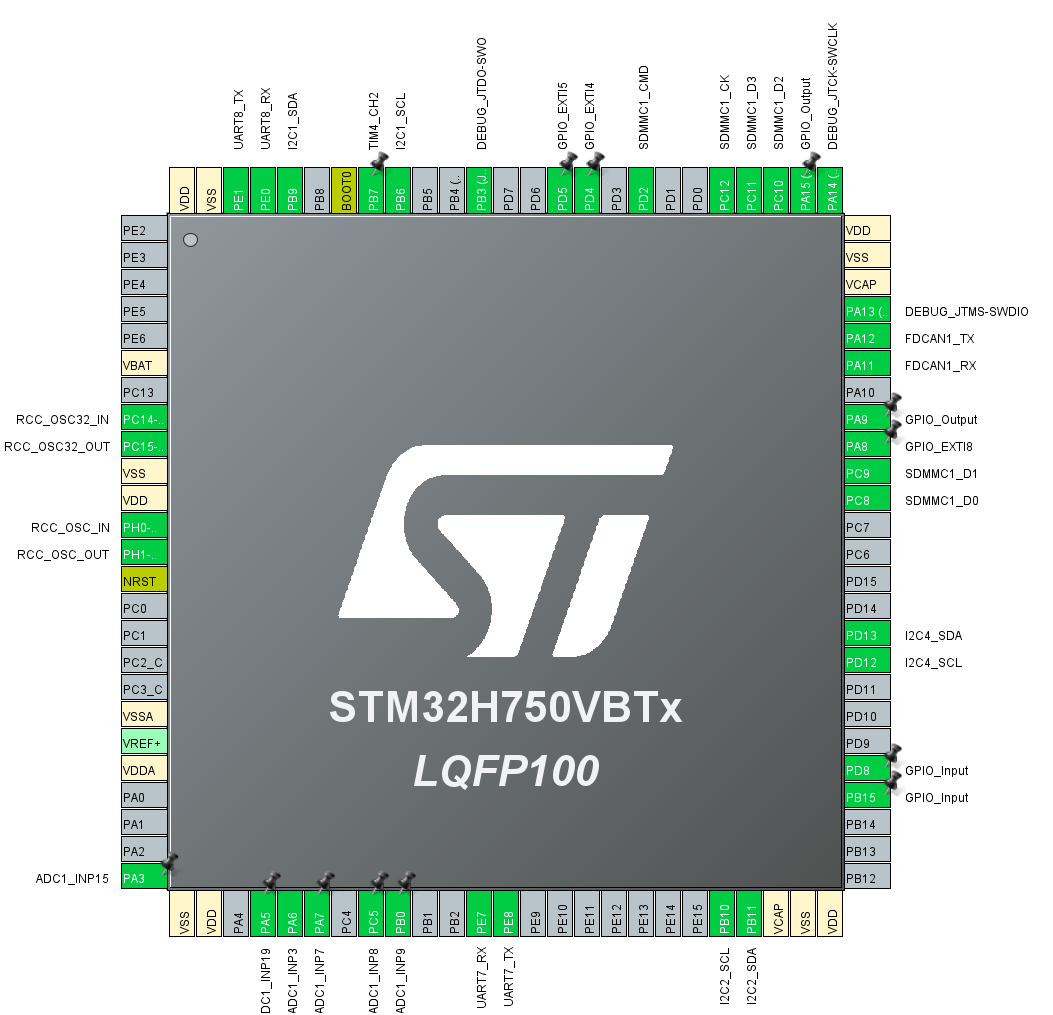
\includegraphics[width=\linewidth]{STMPinout.png}
	\caption{STM32 Pinout}
	\label{fig:STMIOC}
\end{figure}

\paragraph{}
The next major aspect of the schematic design was to ensure that all directional communication signals were connected to the appropriate pins between the microcontroller and the peripherals.
Specifically, it was important to ensure that for both UART connections, the TX pin of the microcontroller was connected to the RX pin of the appropriate component.
On the CAN controller to CAN transceiver connection, though, the opposite needs to occur.
The CAN TX pin on the microcontroller for the CAN controller must be connected to the CAN TX pin of the CAN transceiver and vice versa for RX.
This can be seen in \cref{fig:USBSchematic}, \cref{fig:CANSchematic}, and \cref{fig:STMIOC}.


\begin{figure}[H]
	\centering
	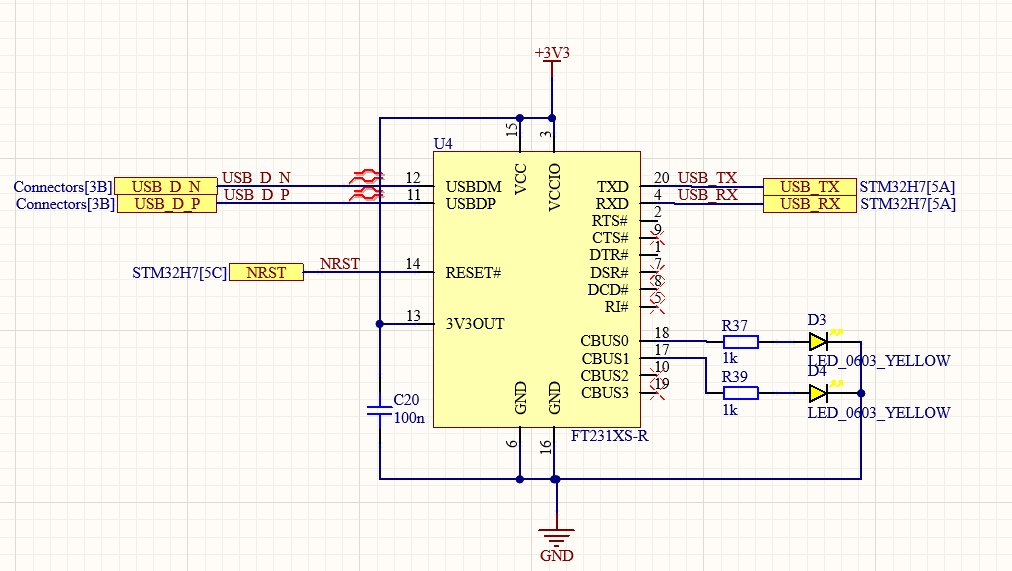
\includegraphics[width=\linewidth]{USBUART.png}
	\caption{USB Transceiver Wiring}
	\label{fig:USBSchematic}
\end{figure}

\begin{figure}[H]
	\centering
	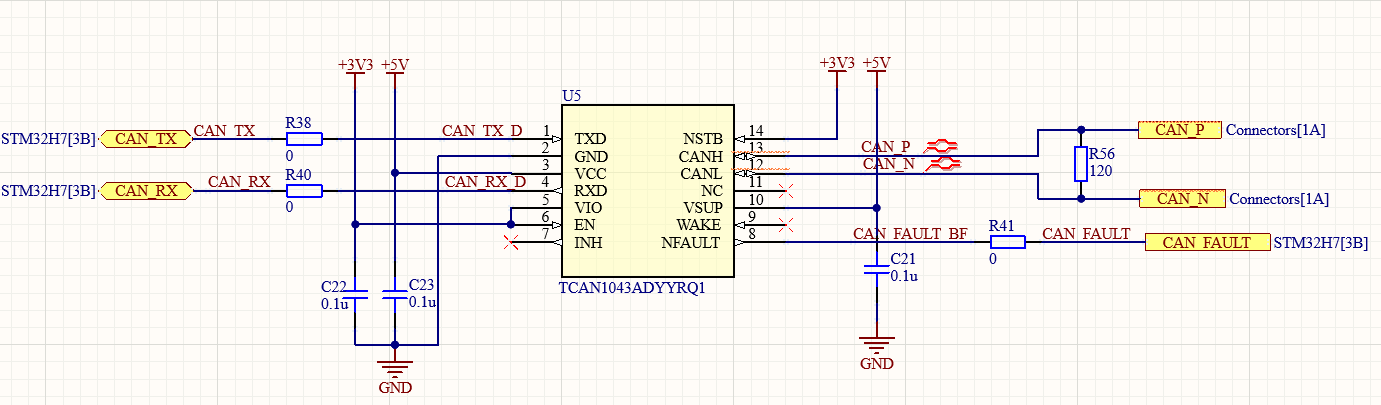
\includegraphics[width=\linewidth]{CAN.png}
	\caption{CAN Transceiver Wiring}
	\label{fig:CANSchematic}
\end{figure}

\paragraph{}
It is also important that pull-up and pull-down resistors are connected to the appropriate signals for communication lines and control signals.
Specifically, pull-up resistors needed to be added for the I2C communication lines as well as the SDIO data lines.
Additionally, the DAQ acts as a terminating node in the CAN network, so the termination resistor for the CAN bus must be present.

\begin{figure}[H]
	\centering
	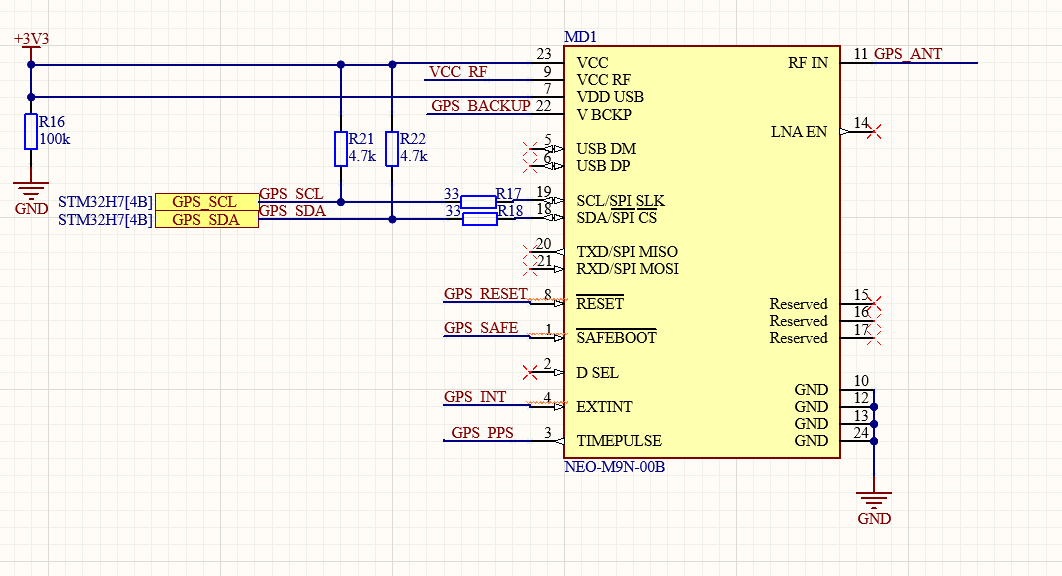
\includegraphics[width=\linewidth]{GPSI2C.png}
	\caption{GPS I2C Wiring}
	\label{fig:I2CSchematic}
\end{figure}

\begin{figure}[H]
	\centering
	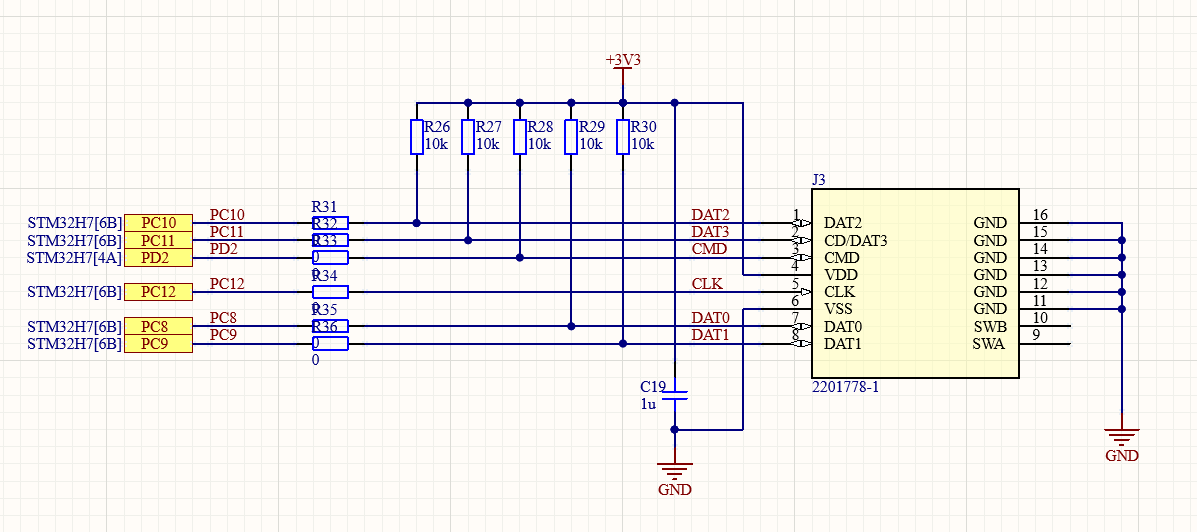
\includegraphics[width=\linewidth]{SDIO.png}
	\caption{Micro SD Reader Wiring}
	\label{fig:SDSchematic}
\end{figure}

\paragraph{}
The final important aspect for this at a system level was to ensure that the controlled impedances of signals were configured if they were needed.
Specifically, the CAN spec and USB spec detail controlled differential impedances for their signals.
As a result, these signals needed to be marked as differential pairs on the schematics as seen in \cref{fig:USBSchematic} and \cref{fig:CANSchematic}.

\subsection{Layout and Routing}

\paragraph{}
Similarly to the schematic design, the layout and routing were mostly outside the scope of this project and were done by another member of the competition team.
However, the layout and routing were reviewed to ensure that a user can effectively interface with the hardware and that all specifications for items such as differential pair impedances were being met.
Additionally, layer stackups, impedance profiles, and rules checks were reviewed to ensure that the PCB would comply with the manufacturer's requirements and tolerances.
The PCBs were manufactured with JLCPCB.
The four layer stackup used for the hardware can be seen in \cref{fig:Stackup}.
There are two signal layers on the top and bottom with two copper planes on the internal layers, one for 3.3V and one for GND.
These internal layers make it easy to provide power and ground to many different places and provide consistent references for differential pairs that exist on the signal layers.

\begin{figure}[H]
	\centering
	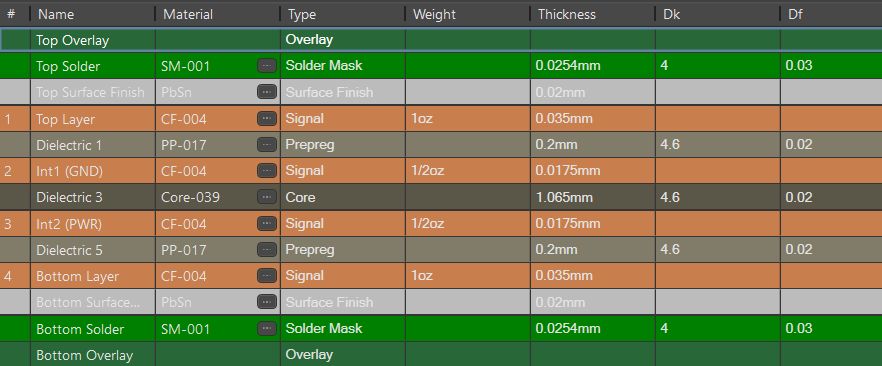
\includegraphics[width=\linewidth]{LayerStackup.png}
	\caption{4 Layer Stackup based on JLCPCB Stackup}
	\label{fig:Stackup}
\end{figure}

\paragraph{}
The CAN spec states that the differential impedance of a CAN bus should be $120 \Omega$.
As can be seen in \cref{fig:CANImpedance}, the impedance of the differential pair will be $120.03 \Omega$, or a less than 0.03\% deviation.
Similarly, the USB spec includes a $90 \Omega$ differential impedance.
As can be seen in \cref{fig:USBImpedance}, the impedance of the differential pair with this profile will be $89.8 \Omega$, or just above a 0.02\% deviation.

\begin{figure}[H]
	\centering
	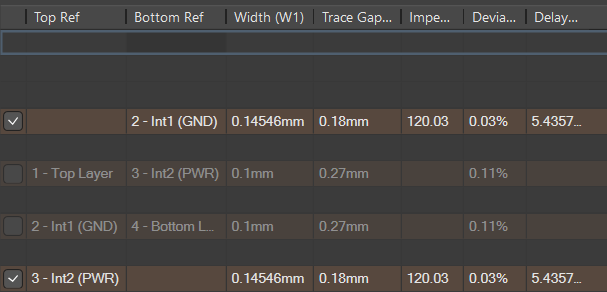
\includegraphics[width=\linewidth]{CANImpedance.png}
	\caption{$120 \Omega$ impedance profile for a 4-layer stackup}
	\label{fig:CANImpedance}
\end{figure}

\begin{figure}[H]
	\centering
	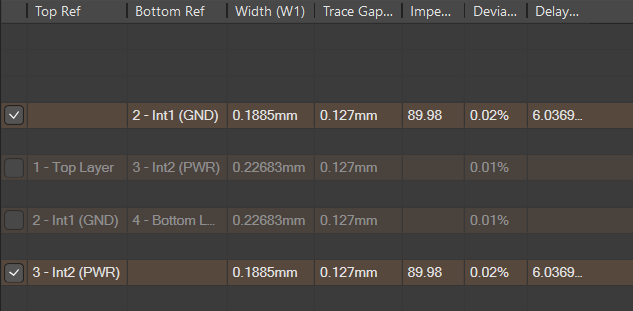
\includegraphics[width=\linewidth]{USBImpedance.png}
	\caption{$90 \Omega$ impedance profile for a 4-layer stackup}
	\label{fig:USBImpedance}
\end{figure}

\paragraph{}
The largest design choice for the layout was to split the hardware into two separate PCBs that could be stacked on top of each other.
The purpose of this was to reduce the overall footprint of the design by utilizing the third dimension.
Due to connector sizes and some large components, the area of a single PCB would have needed to increase significantly, approximately $1750\text{mm}^2$.  By utilizing the third dimension, the total package size was able to decrease by a similar amount.
This is critical for physically mounting the device onto the car, as there is a limited amount of space and few mounting points available.
The way these PCBs attach together can be seen in \cref{fig:PCBAssembly}.

\begin{figure}[H]
	\centering
	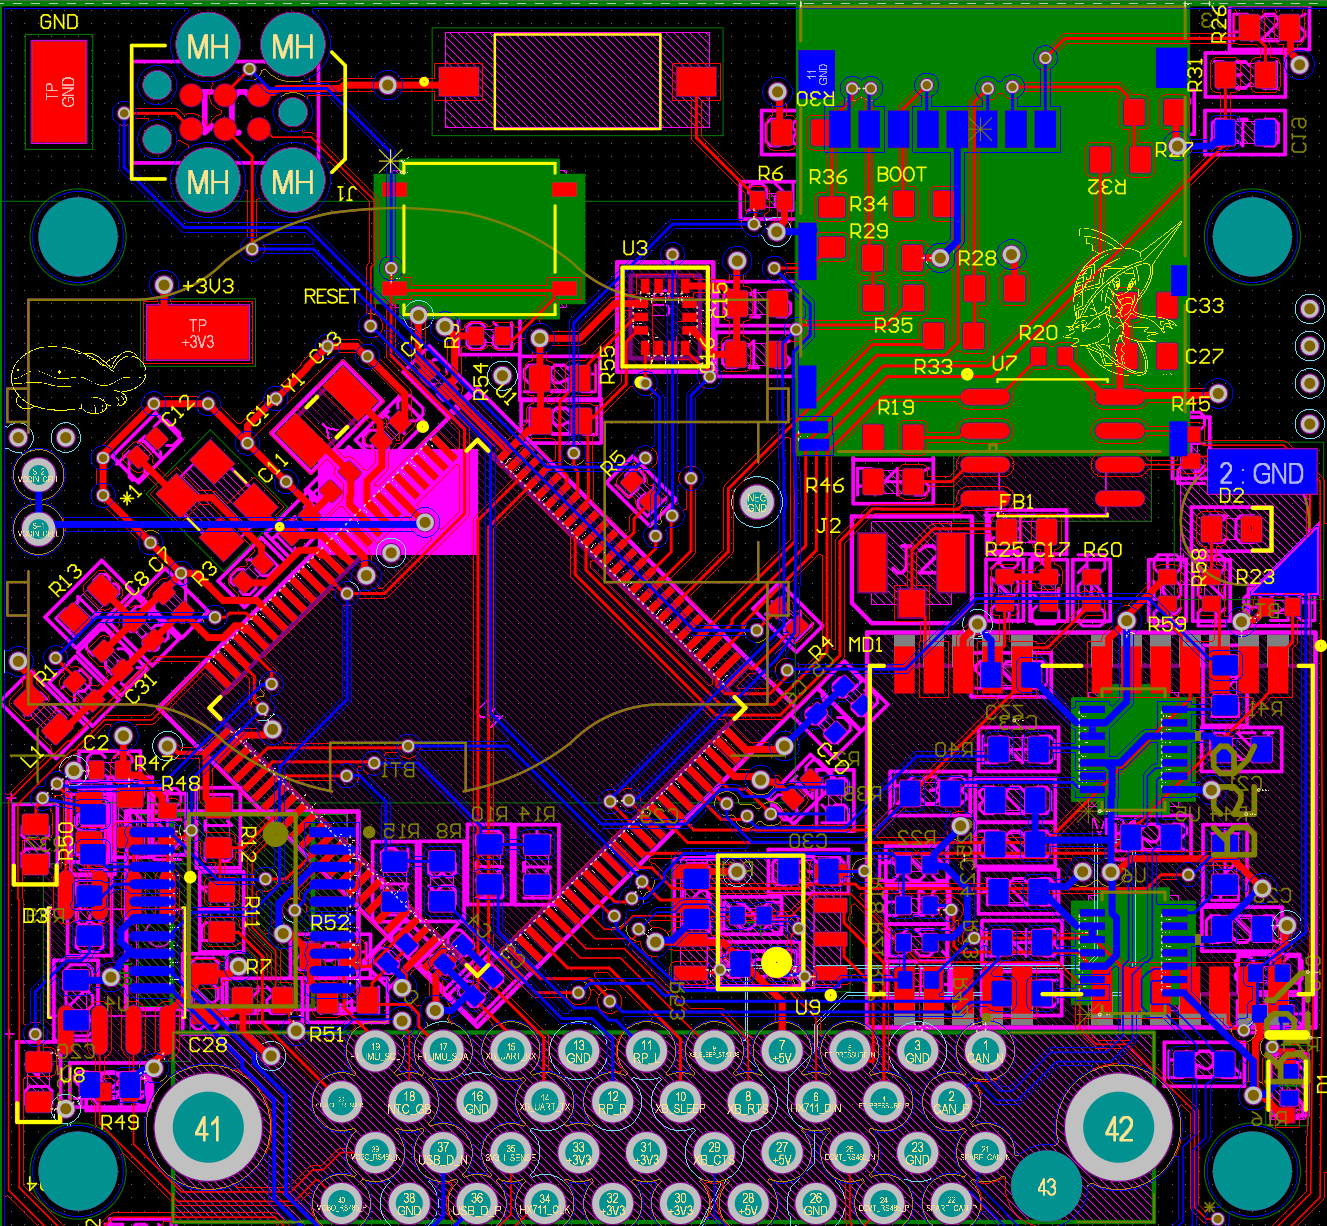
\includegraphics[width=\linewidth]{DAQTOPLayout.png}
	\caption{2D Layout of the top PCB}
	\label{fig:TopLayout}
\end{figure}

\begin{figure}[H]
	\centering
	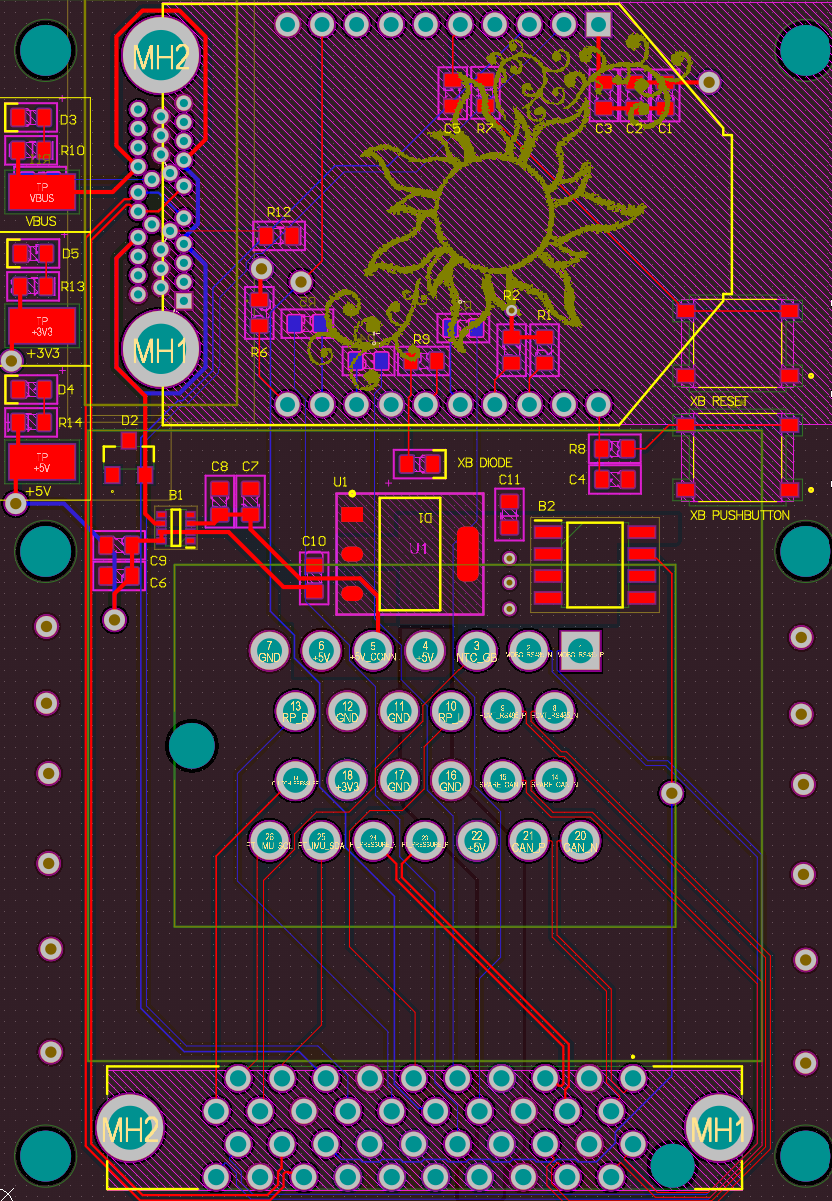
\includegraphics[width=\linewidth]{DAQBaseLayout.png}
	\caption{2D layout of the base PCB}
	\label{fig:BaseLayout}
\end{figure}

\begin{figure}[H]
	\centering
	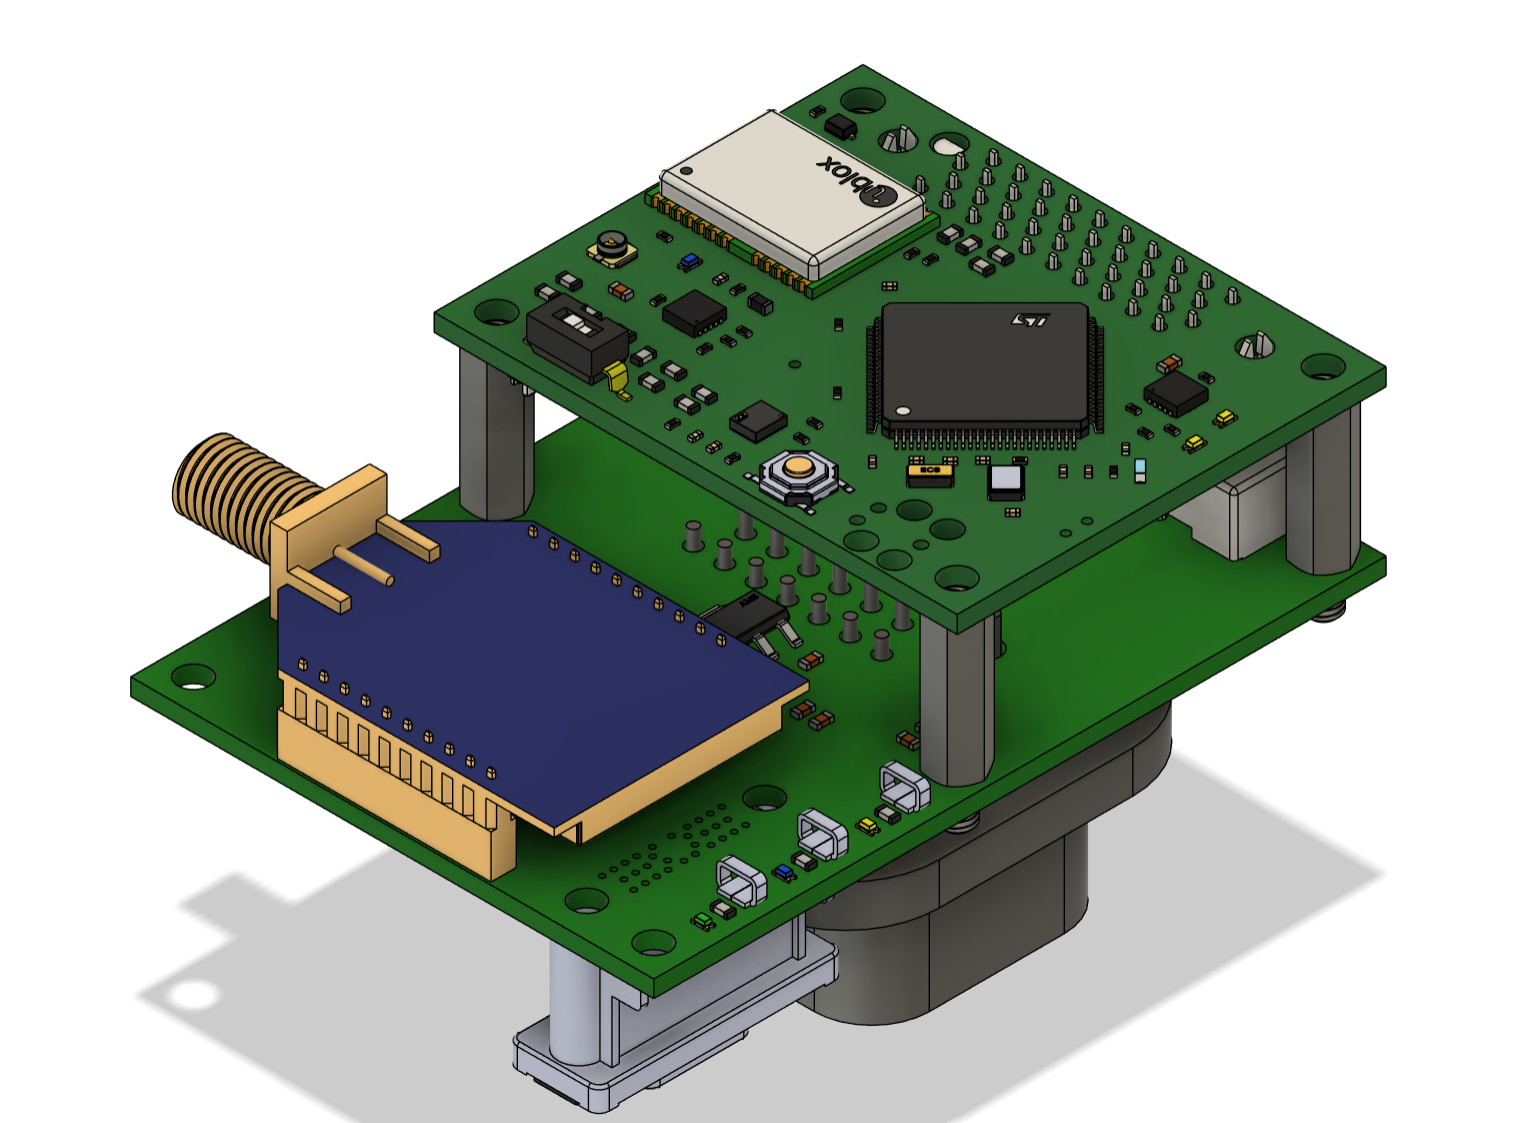
\includegraphics[width=\linewidth]{DAQAssembly.png}
	\caption{3D assembly of the DAQ PCBs}
	\label{fig:PCBAssembly}
\end{figure}

\paragraph{}
The biggest place where component placement is critical is the location of the micro-SD card reader.
This component needs to be placed in a position that, when assembled into an enclosure, the SD card can be inserted into or removed from the reader.
As can be seen in \cref{fig:TopLayout}, the SD card was placed on the edge of the board.
Referencing \cref{fig:PCBAssembly}, this is at the edge next to the radio module, having enough clearance to be able to insert a finger for removal and insertion.